\documentclass{article}

\usepackage{fancyhdr}
\usepackage{extramarks}
\usepackage{amsmath}
\usepackage{amsthm}
\usepackage{amsfonts}
\usepackage{tikz}
\usepackage[plain]{algorithm}
\usepackage{algpseudocode}
\usepackage{enumerate}
\usepackage{amssymb}

\usetikzlibrary{automata,positioning}

%
% Basic Document Settings
%

\topmargin=-0.45in
\evensidemargin=0in
\oddsidemargin=0in
\textwidth=6.5in
\textheight=9.0in
\headsep=0.25in

\linespread{1.1}

\pagestyle{fancy}
\lhead{\hmwkAuthorName}
\chead{\hmwkClass\ (\hmwkClassInstructor\ \hmwkClassTime): \hmwkTitle}
\rhead{\firstxmark}
\lfoot{\lastxmark}
\cfoot{\thepage}

\renewcommand\headrulewidth{0.4pt}
\renewcommand\footrulewidth{0.4pt}

\setlength\parindent{0pt}

%
% Create Problem Sections
%

\newcommand{\enterProblemHeader}[1]{
    \nobreak\extramarks{}{Problem \arabic{#1} continued on next page\ldots}\nobreak{}
    \nobreak\extramarks{Problem \arabic{#1} (continued)}{Problem \arabic{#1} continued on next page\ldots}\nobreak{}
}

\newcommand{\exitProblemHeader}[1]{
    \nobreak\extramarks{Problem \arabic{#1} (continued)}{Problem \arabic{#1} continued on next page\ldots}\nobreak{}
    \stepcounter{#1}
    \nobreak\extramarks{Problem \arabic{#1}}{}\nobreak{}
}

\setcounter{secnumdepth}{0}
\newcounter{partCounter}
\newcounter{homeworkProblemCounter}
\setcounter{homeworkProblemCounter}{1}
\nobreak\extramarks{Problem \arabic{homeworkProblemCounter}}{}\nobreak{}

%
% Homework Problem Environment
%
% This environment takes an optional argument. When given, it will adjust the
% problem counter. This is useful for when the problems given for your
% assignment aren't sequential. See the last 3 problems of this template for an
% example.
%
\newenvironment{homeworkProblem}[1][-1]{
    \ifnum#1>0
        \setcounter{homeworkProblemCounter}{#1}
    \fi
    \section{Problem \arabic{homeworkProblemCounter}}
    \setcounter{partCounter}{1}
    \enterProblemHeader{homeworkProblemCounter}
}{
    \exitProblemHeader{homeworkProblemCounter}
}

%
% Homework Details
%   - Title
%   - Due date
%   - Class
%   - Section/Time
%   - Instructor
%   - Author
%

\newcommand{\hmwkTitle}{Tutorial 5}
\newcommand{\hmwkDueDate}{February 16, 2021}
\newcommand{\hmwkClass}{CZ2003}
\newcommand{\hmwkClassTime}{SS3}
\newcommand{\hmwkClassInstructor}{Assoc Prof Alexei Sourin}
\newcommand{\hmwkAuthorName}{\textbf{Pang Yu Shao}}
\newcommand{\hmwkAuthorID}{\textbf{U1721680D}}

%
% Title Page
%

\title{
    \vspace{2in}
    \textmd{\textbf{\hmwkClass:\ \hmwkTitle}}\\
    \normalsize\vspace{0.1in}\small{Due\ on\ \hmwkDueDate\ at 10:30am}\\
    \vspace{0.1in}\large{\textit{\hmwkClassInstructor\ - \hmwkClassTime}}
    \vspace{3in}\\
    \hmwkAuthorName\\
    \hmwkAuthorID
}

\date{15/02/2021}

\renewcommand{\part}[1]{\textbf{\large Part \Alph{partCounter}}\stepcounter{partCounter}\\}

%
% Various Helper Commands
%

% Useful for algorithms
\newcommand{\alg}[1]{\textsc{\bfseries \footnotesize #1}}

% For derivatives
\newcommand{\deriv}[1]{\frac{\mathrm{d}}{\mathrm{d}x} (#1)}

% For partial derivatives
\newcommand{\pderiv}[2]{\frac{\partial}{\partial #1} (#2)}

% Integral dx
\newcommand{\dx}{\mathrm{d}x}

% Alias for the Solution section header
\newcommand{\solution}{\textbf{\large Solution}}

% Probability commands: Expectation, Variance, Covariance, Bias
\newcommand{\E}{\mathrm{E}}
\newcommand{\Var}{\mathrm{Var}}
\newcommand{\Cov}{\mathrm{Cov}}
\newcommand{\Bias}{\mathrm{Bias}}

\begin{document}

\maketitle

\pagebreak

\begin{homeworkProblem}
    Using rotational sweeping \textbf{clockwise}, define by parametric functions 
    \(x(u,v)\), \(y(u,v)\), \(z(u,v)\), \(u,v \in [0,1]\) the surface displayed in 
    Figure Q1.
    \begin{figure}[H]
        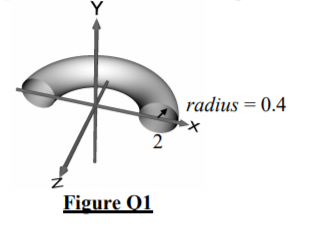
\includegraphics[width=6cm]{fig/q1.PNG}
        \centering
    \end{figure}
    

    \textbf{Solution}\\
    First, get the curve to be swept, curve is a circle with radius \textbf{0.4}, 
    with origin at \textbf{(2,0,0)}.

    This curve can be parametrically defined as:\\
    \(x(u,v) = 2 + 0.4cos(2\pi u)\)\\
    \(x(u,v) = 0.4sin(2\pi u)\)\\
    \(z(u,v) = 0\)
    \\\\
    \begin{figure}[H]
        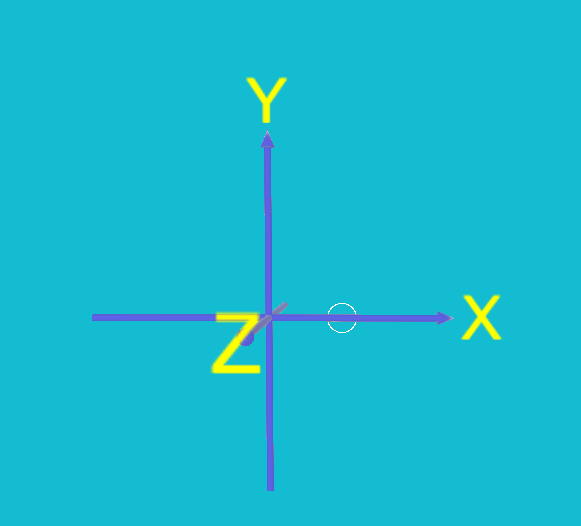
\includegraphics[width=6cm]{fig/q1a.PNG}
        \centering
    \end{figure}
    Next, to sweep the curve along the X-Z plane, we copy the defined function \(x(u,v)\) to 
    \(z(u,v)\) and multiply the function of \(x\) by \(sin(0)\) and the function of \(z\) by 
    \(cos(0)\), and we obtain the following functions and curve:\\
    \(x(u,v) = (2 + 0.4cos(2\pi u))sin(0)\)\\
    \(x(u,v) = 0.4sin(2\pi u)\)\\
    \(z(u,v) = (2 + 0.4cos(2\pi u))cos(0)\)
    \\
    \begin{figure}[H]
        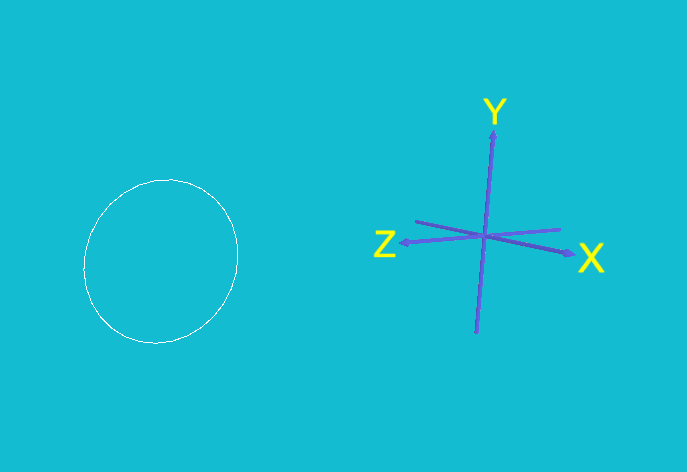
\includegraphics[width=6cm]{fig/q1b.PNG}
        \centering
    \end{figure}
    We can see from the figure above that the curve is lying on the Z-axis, however it needs to begin
    from the negative X-axis and swept clockwise, In order to get the correct starting location for sweeping 
    to begin, we introduce an offset of \(\mathbf{-\frac{\pi}{2}}\) to the sin/cos functions:\\
    \(x(u,v) = (2 + 0.4cos(2\pi u))sin(-\frac{\pi}{2})\)\\
    \(x(u,v) = 0.4sin(2\pi u)\)\\
    \(z(u,v) = (2 + 0.4cos(2\pi u))cos(-\frac{\pi}{2})\)\\
    \begin{figure}[H]
        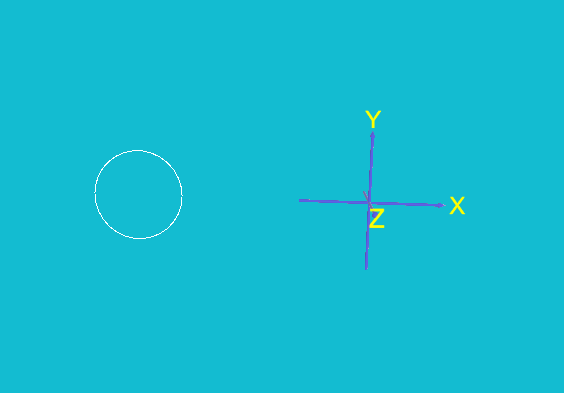
\includegraphics[width=6cm]{fig/q1c.PNG}
        \centering
    \end{figure}
    Lastly, we perform the sweeping to produce the surface. This is done by introducing the variable \(\mathbf{v}\) into 
    the sin/cos functions, multiplied by \(-\pi\) for the clockwise sweeping from negative x-axis to positive x-axis.\\
    \(\mathbf{x(u,v) = (2 + 0.4cos(2\pi u))sin(-\frac{\pi}{2} - \pi v)}\)\\
    \(\mathbf{x(u,v) = 0.4sin(2\pi u)}\)\\
    \(\mathbf{z(u,v) = (2 + 0.4cos(2\pi u))cos(-\frac{\pi}{2} - \pi v})\)\\
    \(u,v \in [0,1]\)
    \begin{figure}[H]
        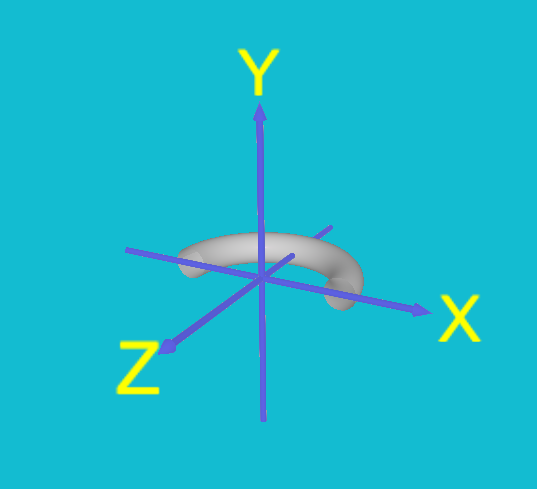
\includegraphics[width=6cm]{fig/q1d.PNG}
        \centering
    \end{figure}




\end{homeworkProblem}
\pagebreak
\begin{homeworkProblem}
    Write parametric equations \(x(u,v)\), \(y(u,v)\), \(z(u,v)\), \(u,v \in [0,1]\) 
    defining the surface created by sweeping (\textbf{clockwise} rotation by \(3\pi /2\) 
    and vertical displacement by \textbf{-2}) of the curve which is defined in polar 
    coordinates by \(r = 0.5sin(4\alpha), \alpha \in [0, 2\pi]\) (Figure Q2).
    \begin{figure}[H]
        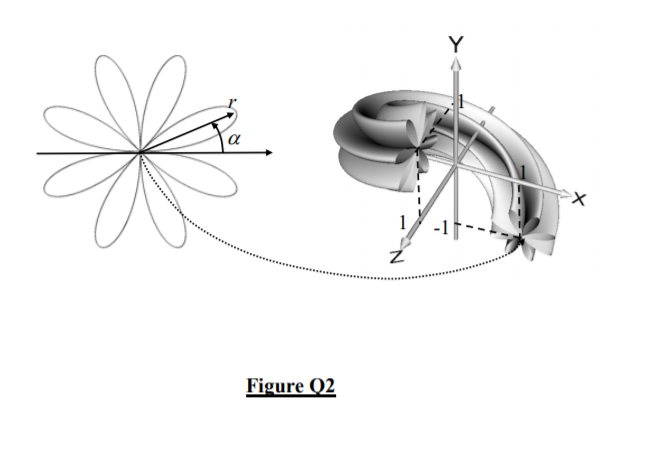
\includegraphics[width=10cm]{fig/q2.PNG}
        \centering
    \end{figure}

    \textbf{Solution}\\
    First, convert definition of curve from polar coordinates to cartesian coordinates.\\
    \(x = r\ cos(\alpha)\)\\
    \(y = r\ sin(\alpha)\)\\

    \(x(u,v) = 0.5sin(8\pi u)cos(2\pi u)\)\\
    \(y(u,v) = 0.5sin(8\pi u)sin(2\pi u)\)\\
    \(z(u,v) = 0\)
    \begin{figure}[H]
        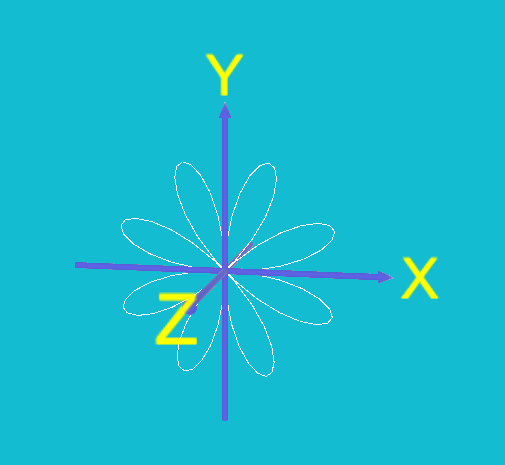
\includegraphics[width=6cm]{fig/q2a.PNG}
        \centering
    \end{figure}

    Next, we add x and y offsets of 1, which is needed for to shift the curve to the start position
    of the sweeping\\
    \(x(u,v) = 1+ 0.5sin(8\pi u)cos(2\pi u)\)\\
    \(y(u,v) = 1+ 0.5sin(8\pi u)sin(2\pi u)\)\\
    \(z(u,v) = 0\)
    \begin{figure}[H]
        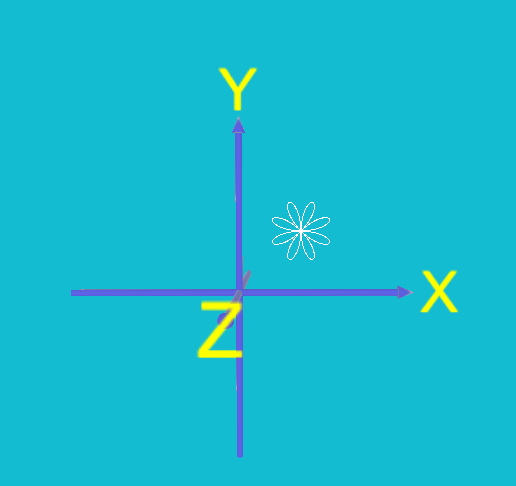
\includegraphics[width=6cm]{fig/q2b.PNG}
        \centering
    \end{figure}


    Next, to sweep the curve along the X-Z plane, we copy the defined function \(x(u,v)\) to 
    \(z(u,v)\) and multiply the function of \(x\) by \(sin(0)\) and the function of \(z\) by 
    \(cos(0)\), and we obtain the following functions and curve:\\
    \(x(u,v) = (1+ 0.5sin(8\pi u)cos(2\pi u))sin(0)\)\\
    \(y(u,v) = 1+ 0.5sin(8\pi u)sin(2\pi u)\)\\
    \(z(u,v) = (1+ 0.5sin(8\pi u)cos(2\pi u))cos(0)\)
    \begin{figure}[H]
        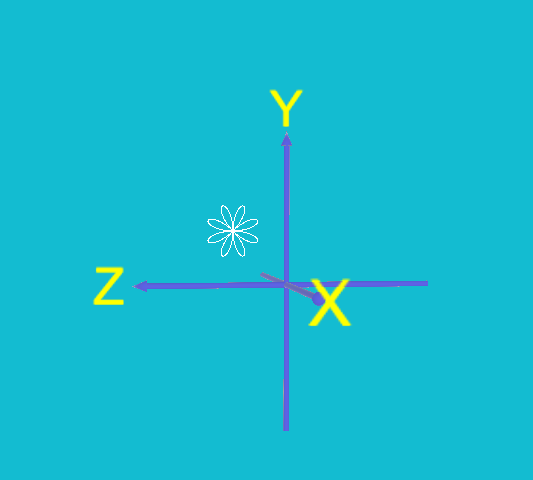
\includegraphics[width=6cm]{fig/q2c.PNG}
        \centering
    \end{figure}

    Lastly, to perform the clockwise sweep, we add \((-3\pi/2)v\) as the argument of the sin/cos functions of 
    the X and Z functions. The vertical sweep component can be done by adding \(-2v\) to the Y funciton. We thus 
    end up with the following:\\
    \(\mathbf{x(u,v) = (1+ 0.5sin(8\pi u)cos(2\pi u))sin((-3\pi/2)v)}\)\\
    \(\mathbf{y(u,v) = 1 + 0.5sin(8\pi u)sin(2\pi u) - 2v}\)\\
    \(\mathbf{z(u,v) = (1+ 0.5sin(8\pi u)cos(2\pi u))cos((-3\pi/2)v)}\)\\
    \(u,v \in [0,1]\)

    \begin{figure}[H]
        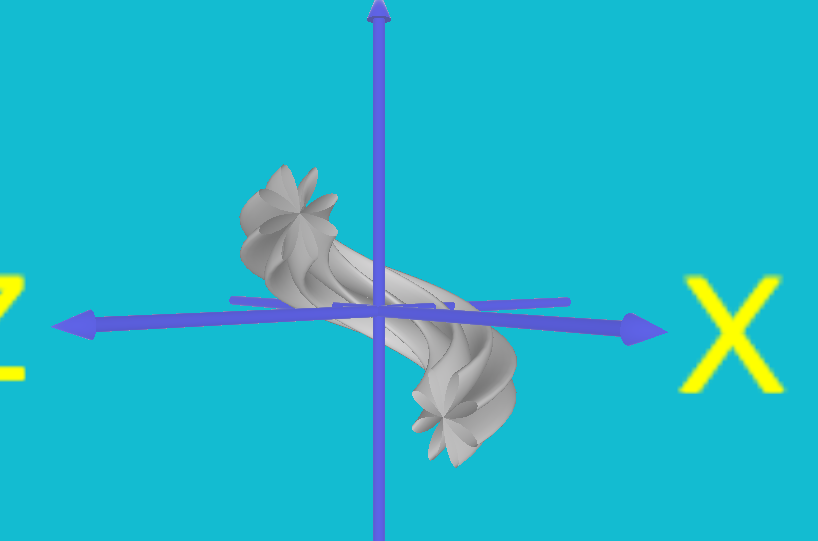
\includegraphics[width=6cm]{fig/q2d.PNG}
        \centering
    \end{figure}
    
\end{homeworkProblem}




\end{document}